\documentclass[11pt,a4paper]{article}

\usepackage[utf8x]{inputenc}   % omogoča uporabo slovenskih črk kodiranih v formatu UTF-8
\usepackage[slovene]{babel}    % naloži, med drugim, slovenske delilne vzorce

\usepackage[hyphens]{url}
\usepackage{hyperref}

\usepackage{graphicx}


\title{Akcijski načrt za mojo diplomsko nalogo:\\
``naslov diplomskega dela''}
\author{Ime Priimek\\
e-naslov\\
\ \\
predvideni MENTOR: (viš. pred./doc./prof.) dr. X Y \\
Fakulteta za računalništvo in informatiko Univerze v Ljubljani
\date{\today}         
}



\begin{document}
\maketitle

\section{Katere aktivnosti so potrebne za izdelavo moje diplomske naloge}

Sestavi seznam (itemize) aktivnosti, ki so potrebne, da lahko uspešno dokončam svoje zastavljeno diplomsko delo.

Za vsako aktivnost na kratko, v nekaj stavkih opiši, kako bo potekala in kakšen bo končen rezultat aktivnosti (angl. deliverable).

Po potrebi vsako aktivnost še razdeli na podaktivnosti in sestavi podseznam!

Kako se boš lotil delitve problema na aktivnosti?

Pri opisu aktivnosti bodi kar se da konkreten!





\section{Kako so identificirane aktivnosti povezane med seboj}

Nariši mrežni diagram v primernem grafičnem orodju, npr. \url{https://www.genmymodel.com/activity-diagram-online},
da prikažeš medsebojno odvisnost med aktivnostmi. Katere so začetne, katere končne, vrstni red in morebitno paralelno izvajanje aktivnosti!


Na sliki \ref{sl:mreza} je mrežni diagram za izdelavo moje diplomske naloge.

\begin{figure}[htb]
\centerline{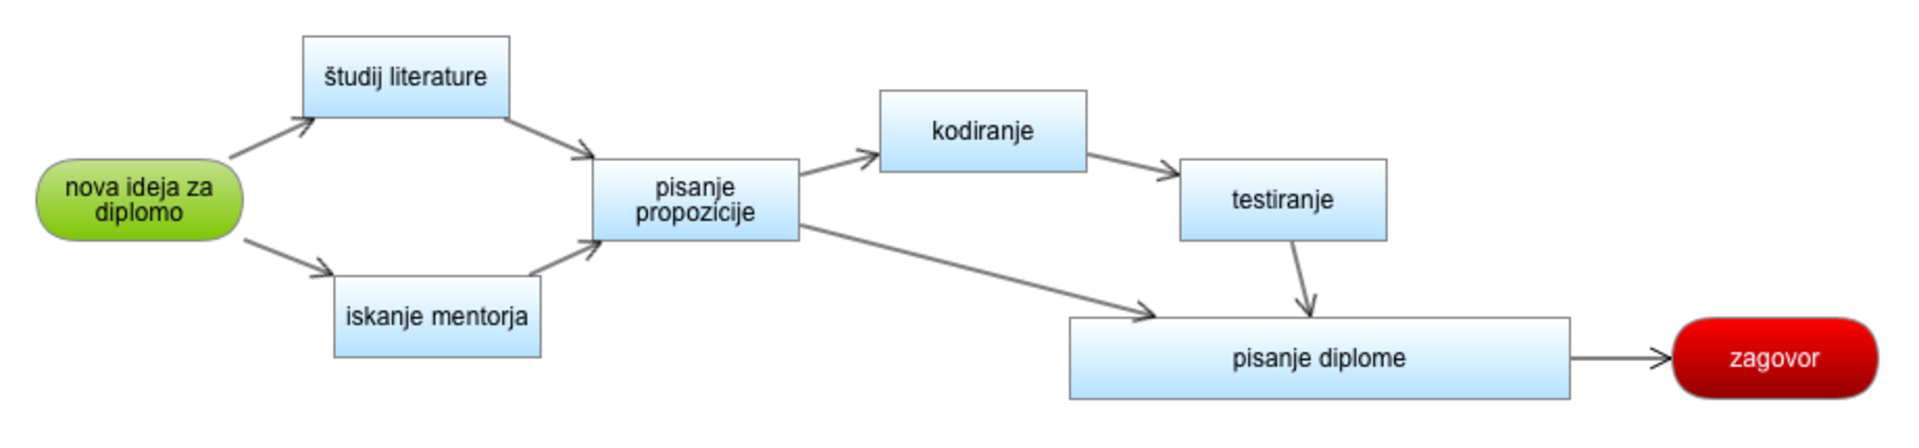
\includegraphics[width=1.0\textwidth]{mreza.pdf}}
\caption{Mrežni diagram aktivnosti za mojo diplomsko nalogo.}
\label{sl:mreza}
\end{figure}


\section{Časovna analiza in optimizacija načrta}

Oceni čas trajanja posameznih aktivnosti.
Seštej ocene, da prideš do časa trajanja celotnega projekta.

Ali je ocenjeni čas trajanja primeren? Ali ga moraš skrajšati? Katere aktivnosti boš skrajšal, da boš diplomo lahko pravočasno končal?

Katere so kritične aktivnosti?


\section{Akcijski načrt}

Kaj boš najprej naredil, da se bo projekt začel izvajati?



\end{document}  




